\documentclass{article}
\usepackage[utf8]{inputenc}
\usepackage{mathtools}
\usepackage{titlesec}
\usepackage{indentfirst}
\usepackage{graphicx}
\usepackage{float}


\graphicspath{{PCAPics/}}
\everymath{\displaystyle}
\setcounter{secnumdepth}{4}

\title{Folosirea PCA pentru recunoasterea imaginilor cu ajutorul librariei Accord}
\author{Motrescu Radu}
\date{}

\begin{document}

\maketitle

\newpage

\tableofcontents

\newpage

\section{Libraria Accord.NET}
Libraria Accord.Net contine clase pentru:
\begin{itemize}
\item Calcul stiintific: matematica, statistica si machine learning
\item Procesare de imagini si semnale: imagini, semnale audio si recunoastere si urmarire faciala in timp real
\item Librarii suport pentru controale specifice: histograme, scatter-plots, controale pentru fiecare clasa de procesare imagini si semnale
\end{itemize}


In contextul cerintelor pe care vrem noi sa le indeplinim, vom folosi clase dedicate matematicii, statisticii, si ale unor controale de afisare a datelor. 

\newpage

\section{Ce este PCA?}
PCA, sau Principal Component Analysis, sau pe romaneste, Analiza Componentelor Principale este o unealta matematica aplicata din algebra liniara.

Este o metoda non-parametrica (care nu depinde de statistici) de a extrage informatiile relevante dintr-un set de date complex sau confuz.

\paragraph{Un scurt exemplu: }
Sa presupunem ca am extras informatii pentru 100 de parametri pentru un student: inaltime, varsta, greutate, nota obtinuta la un test, culoarea parului etc. Vrem sa gasim cele mai importante caracteristici care definesc studentul. Cum facem asta? Folosim PCA pentru a selecta numai cele mai importante caracteristici.

\begin{itemize}
	\item Ce parametri dorim sa indepartam:
	\begin{itemize}
	\item Constanti: numarul de capete, care este 1 pentru toti studentii
	\item Aproape constanti: grosimea firului de par: 0.003, 0.002, 0.0005 etc.
	\item Care depind de alti parametri
	\end{itemize}
	\item Ce parametri dorim sa pastram:
	\begin{itemize}
	\item Care nu depind de alti parametri: culoarea ochilor
	\item Care se schimba mult, au variatie mare: notele
	\end{itemize}
\end{itemize}

A putea elimina parametrii irelevanti si a-i pastra pe cei relevanti este usor pentru un om, el putand vedea clar care parametri nu exprima informatii relevante despre subiectul respectiv, dar cum putem face calculatorul sa isi dea seama de acesti parametri? Folosind matematica, desigur!

Dorim sa minimizam "sunetul de fundal" si redundanta datelor si sa maximizam variatia dintre parametri.

Se poate vedea in imaginea de mai jos maximizarea variatiei dintre axele norului de puncte respectiv.

\begin{figure}[H]
\centering
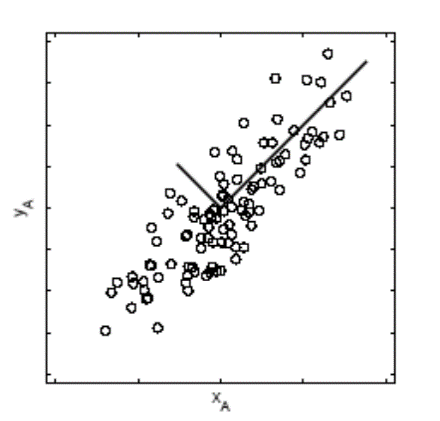
\includegraphics[scale=0.5]{Picture1}
\end{figure}

In imaginile de mai jos se pot vedea inregistrarile unor informatii. In imaginea (a) si (b) se poate vedea cum informatiile nu sunt corelate, avand redunanta mica spre medie (ex: inaltimea unui student si media lui), iar in imaginea (c) se poate vedea o redundanta mare, insemnand ca ambii parametrii pot fi exprimati unul in functie de celalalt.

\begin{figure}[H]
\centering
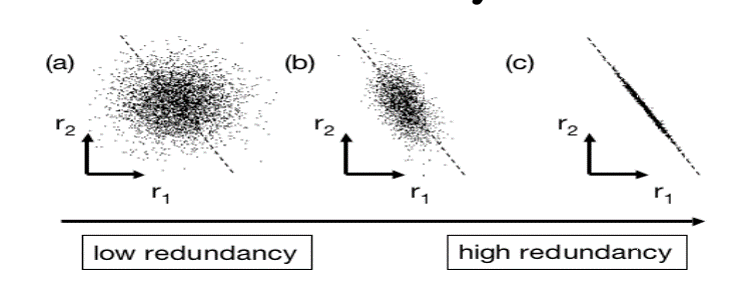
\includegraphics[width=\linewidth]{Picture2}
\end{figure}

\paragraph{Variatia} Este un mijloc de realizare a variabilitatii datelor dintr-un set de date cu media $\overline{X}$:

\begin{equation}
\sigma^2=\frac{\sum_{i=1}^{n} \left( X_i - \overline{X} \right)^2 }{n-1}
\end{equation}

\paragraph{Covariatia} Reprezinta variabilitatea fiecarei dimensiuni in relatie cu celelalte, si este masurata intre 2 dimensiuni pentru a se putea observa relatia dintre cele 2, spre exemplu numarul de ore studiate si nota obtinuta la examen.

\begin{equation}
\text {var} \left( X \right) = \frac{\sum_{i=1}^{n} \left( X_i - \overline{X} \right) \left( X_i - \overline{X} \right) }{n-1}
\end{equation}


\begin{equation}
\text {cov} \left( X,Y \right) = \frac{\sum_{i=1}^{n} \left( X_i - \overline{X} \right) \left( Y_i - \overline{Y} \right) }{n-1}
\end{equation}


\paragraph{Matricea de covariatie}
Consideram setul de date din care extragem valoarea medie (zero-mean data) si avand setul de vectori \( \left\{ x_1, x_2, ..., x_m \right\} \) care reprezinta liniile unei matrici $X_{m,n}$.

Fiecare linie a matricii reprezinta toate masuratorile unui anumit parametru, iar fiecare coloana reprezinta masuratorile care s-au intamplat la un moment dat.

De aici ajungem la definitia matricei de covariatie:

\begin{equation}
S_x \equiv \frac{1}{n-1}XX^T \text { where } X = 
\begin{bmatrix}
x_1 \\ \vdots \\ x_m
\end{bmatrix}
\end{equation}

$S_x$ este o matrice simetrica $m \times m$, termenii de pe diagonala reprezentand variatia din acelasi parametru, iar termenii care nu sunt de pe diagonala reprezinta covariatia dintre parametri diferiti. Calculand $S_x$, cuantificam corelatia dintre toate posibilele perechi de masuratori. Observand elementele din matrice, o cavariatie mare reprezinta un caz de redundanta mare, iar o covariatie egala cu 0 reprezinta date complet necorelate.

\begin{equation}
C=\begin{bmatrix}
cov(X,X) && cov(X,Y) && cov(X,Z) \\
cov(Y,X) && cov(Y,Y) && cov(Y,Z) \\
cov(Z,X) && cov(Z,Y) && cov(Z,Z)
\end{bmatrix}
\end{equation}


\paragraph{Valorile si vectorii proprii}
Urmatorul pas in calcularea PCA este aflarea valorilor si a vectorilor proprii ale matricii de covariatie. Extragand aceste informatii, ele ne vor arata componentele principale ale setului de date: vectorul propriu cu cea mai mare valoare proprie este componenta principala a setului de date. Se obisnuieste sortarea vectorilor proprii in functie de valoarea proprie pentru a determina ordinea de semnificativitate.

Vectorii si valorile proprii reies din probleme de urmatoarea forma:
\begin{equation}
A.v= \lambda . v
\end{equation}

\textbf{A}: matrice $m \times m$


\textbf{v}: vector $m \times 1$  nenul


$\lambda$: constanta

Pentru orice valoare a lui $\lambda$ pentru care ecuatia are solutie se numeste valoarea proprie a lui A, si vectorul \textbf{v} care corespunde acestei valori se numeste vectorul propriu a lui A.

\paragraph{Pasul final PCA} este sa aflam valorile finale ale setului de date. Aici avem optiunea sa ignoram o parte din dimensiunile pe care le avem, deoarece ele pot fi nesemnificative, avand valori proprii mici, sau dorim afisarea lor in 1, 2 sau 3 dimensiuni. Dupa stabilirea vectorilor proprii doriti, aflarea datelor finale este simpla, proiectam punctele in spatiul lor: 

FinalData = RowFeatureVector $\times$ RowZeroMeanData

\textbf{RowFeatureVectore} este matricea cu vectorii proprii transpusi, cu cel mai semnificati vector propriu pe prima linie.

\textbf{RowZeroMeanData} este matricea care contine setul de date initial din care s-a scazut valorea medie.

Matricea rezultata \textbf{FinalData} va contine setul de date dupa aplicarea algoritmului PCA.
\newpage

\section{Jurnalul dezvoltarii aplicatiei}

\subsection{Aplicatia AccordPCA}
Primii pasi pe care i-am facut in cadrul acestui proiect a fost implementarea algoritmului PCA. Acest lucru a fost realizat usor, folosind libraria Accord, mai specific, pentru a realiza diferitele operatii cu matrici. 

\begin{figure}[H]
\centering
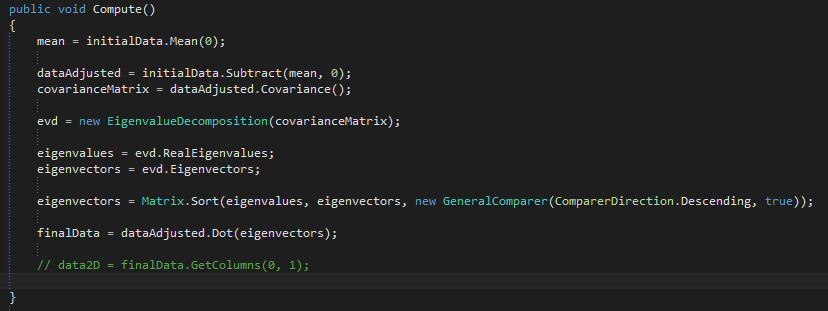
\includegraphics[width=\linewidth]{Compute}
\end{figure}

Pentru a testa acest algoritm, am introdus prima data un set de date deja testat de catre altcineva, unde se poate observa clar rezultatul algoritmului. ( referinta catre http://dai.fmph.uniba.sk/courses/ml/sl/PCA.pdf) 
\begin{figure}[H]
\centering
\caption{Primul test PCA}
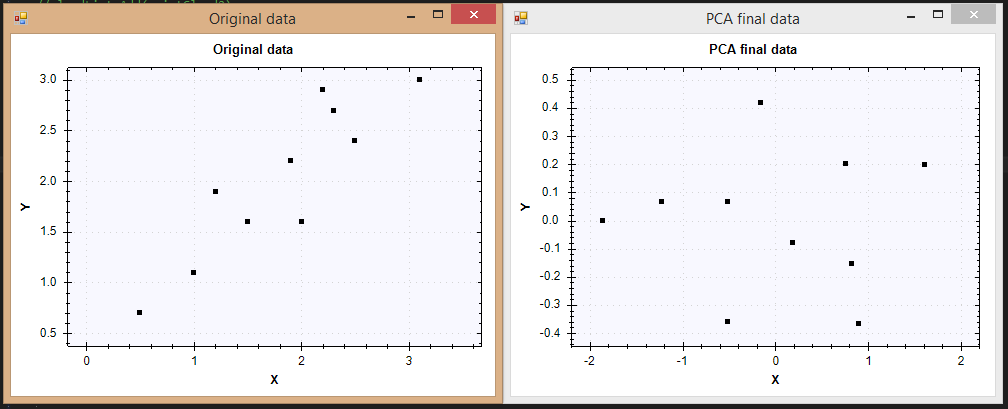
\includegraphics[width=\linewidth]{Test1}
\end{figure}
\newpage

Urmatorul lucru pe care l-am dorit sa il facem a fost sa vedem cum mai multe noruri de puncte, de diferite dimensiuni, se modifica dupa aplicarea algoritmului. Pentru acest lucru, am creat o clasa \textbf{PointCloud} care descrie un nor de puncte. In interiorul clasei am generat norul de puncte in jurul unor coordonate $\left(x,y\right)$, sub forma unui disc, in care punctele au distributie normala. Rezultatele au fost urmatoarele:

\begin{figure}[H]
\centering
\caption{Al doilea test PCA}
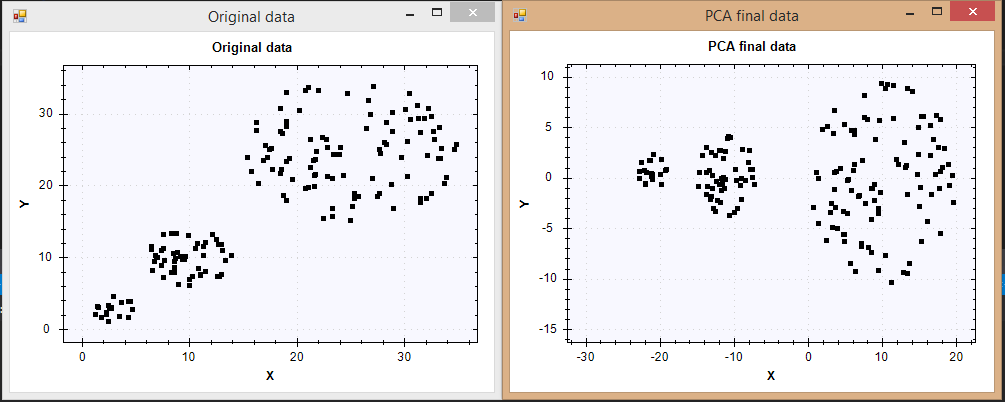
\includegraphics[width=\linewidth]{Test2}
\end{figure}

La fel ca in primul test, se poate observa aranjarea dupa prima componenta principala a norilor.


\subsection{Aplicatia PlotPCA}
In acest moment, am decis sa realizam o aplicatie care are un GUI usor de folosit si unde fiecare nor de puncte este reprezentat in alta culoare, pentru a se vedea mai clar ce se intampla, acest lucru fiind mai important pentru seturile de date in care masuratorile pentru fiecare entitate sunt intrepatrunse.

\subsubsection{Setul 3-cloud-points}
Primele teste pe care le-am facut, au fost pe 3 nori de puncte generati aleator, la fel ca in exemplul de mai sus, si se poate vedea mai clar separarea norilor atat pe in spatiu 2D, cat si pe axa primei componente, cea cu cea mai mare variatie. De asemenea, atunci cand norii se suprapun putin de-a lungul axei Y, algoritmul PCA reuseste sa separe norii complet de-a lungul axei primei componente. Pe de alta parte, daca norii se suprapun mai mult, atunci se poate observa ca algoritmul PCA nu mai poate separa norii la fel de bine ca si pana acum.

\begin{figure}[H]
\centering
\caption{Nori separati total}
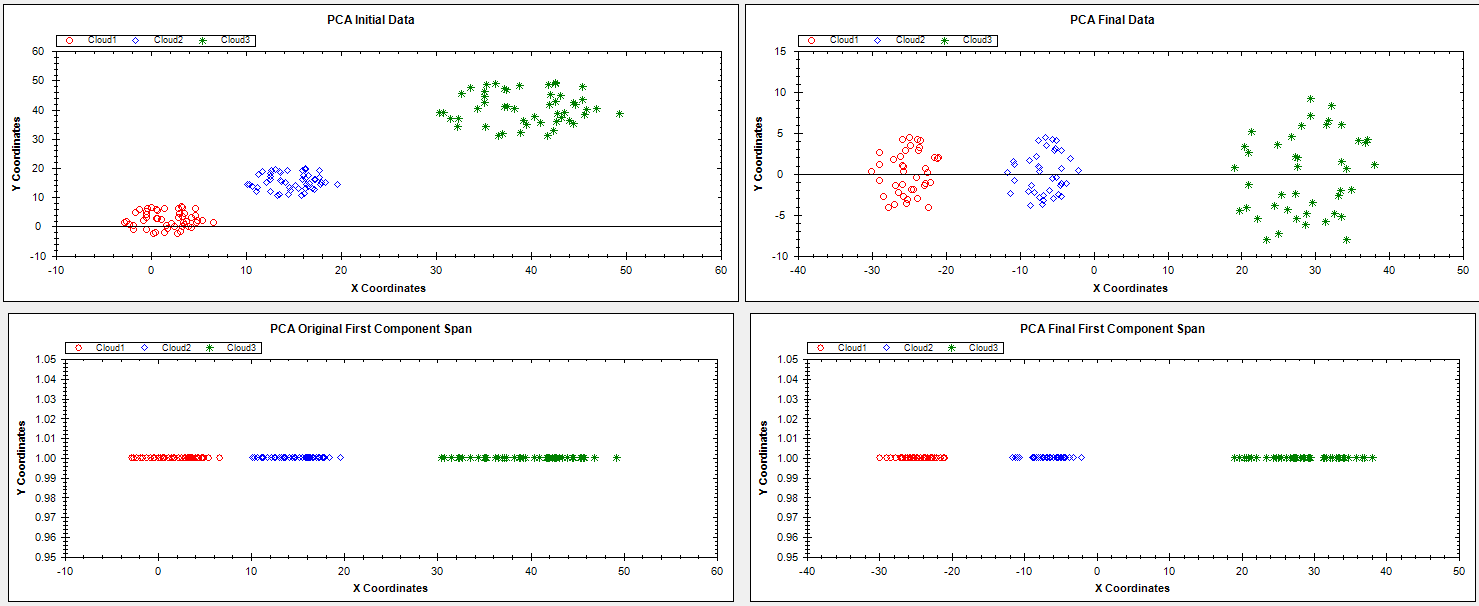
\includegraphics[width=\linewidth]{threecloud1}
\end{figure}


\begin{figure}[H]
\caption{Nori interesectati partial}
\centering
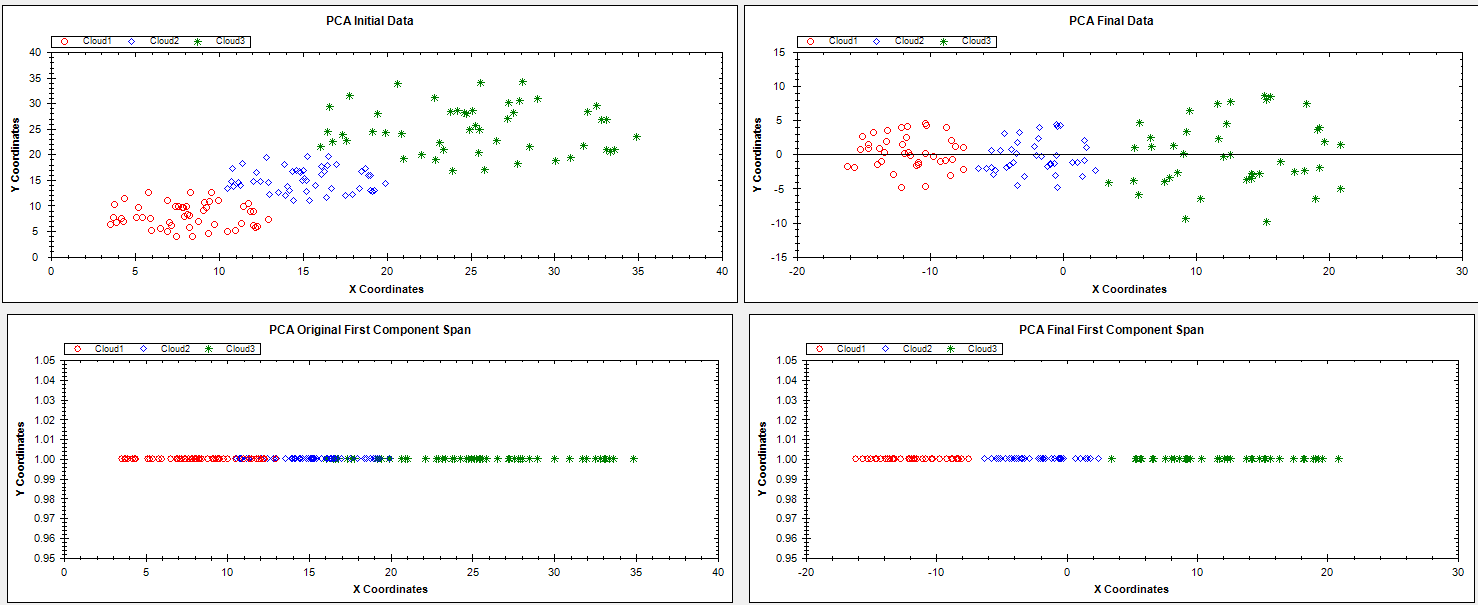
\includegraphics[width=\linewidth]{threecloud2}
\end{figure}


\begin{figure}[H]
\centering
\caption{Norul albastru si verde intersectati aproape total}
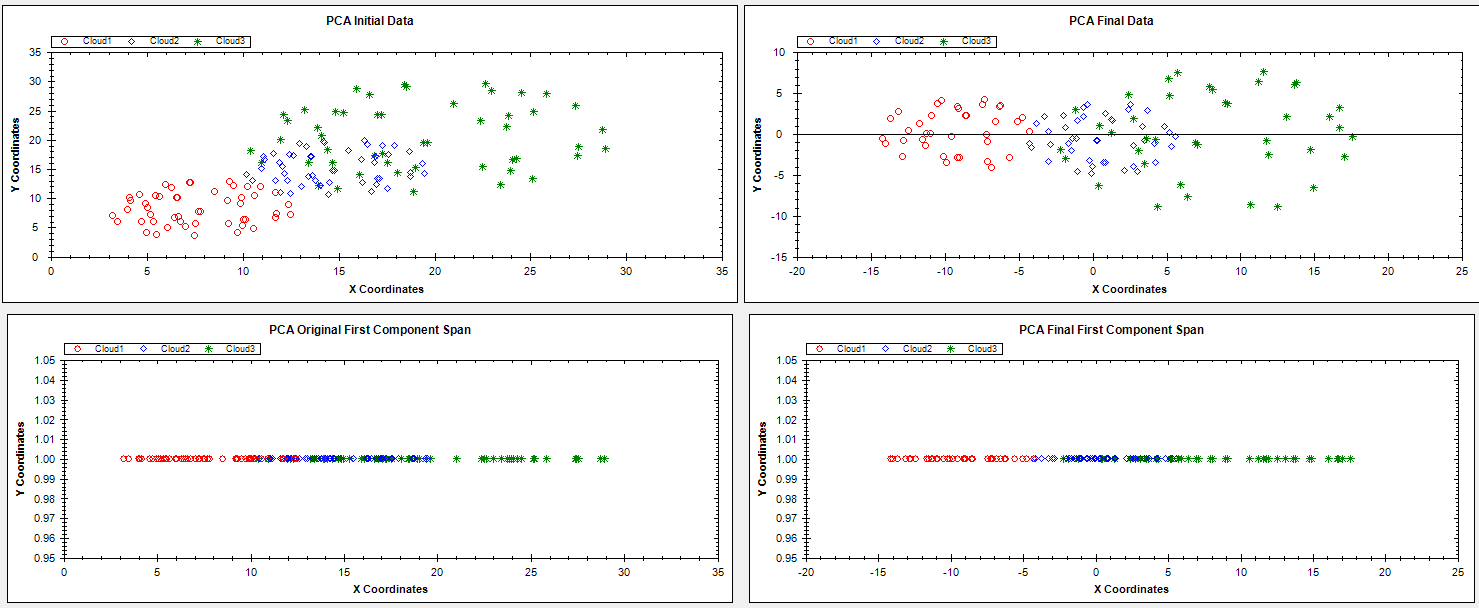
\includegraphics[width=\linewidth]{threecloud3}
\end{figure}


\subsubsection{Setul two-moon si abordarea Kernel PCA}
Pentru a aborda problema seturilor de date liniar inseparabile, nu putem folosi abordarea PCA simpla, rezultatul nu va fi cel dorit, dupa cum se poate vedea aplicand algoritmul PCA pentru setul two-moon: cele doua seturi de puncte se amesteca de-a lungul primei componente principale, astfel o clasificare a unui nou punct proiectat in spatiul respectiv va fi dificila, deoarece nu putem seta un punct de delimitare intre cei doi nori, acestia fiind intrepatrunsi.

Abordarea Kernel PCA rezolva acest lucru prin proiectarea datelor intr-un spatiu dimensional mai mare, unde ele vor deveni liniar separabile, iar acest lucru se face cu o "functie kernel".

Pentru a implementa Kernel PCA, vom avea in considerare urmatoarele 2 lucruri:

\textbf{1. Calcularea matricii kernel} 

Pentru fiecare pereche de puncte se calculeaza :

\begin{equation}
k(x_i,x_j)=\exp(-\gamma \|x_i - x_j\|_2^2)
\end{equation}

Daca avem un set de date cu 100 de mostre, matricea kernel va fi o matrice simetrica $100 \times 100$.

Alegerea valorii lui $\gamma$ este foarte importanta, in functie de ea rezultatul va fi cel dorit sau nu.

\textbf{2. Calcularea vectorilor si a valorilor proprii}

Deoarece nu putem garanta ca matricea e centrata, vom aplica urmatoarea formula pentru a o centra: 

\begin{equation}
K'=K-1_NK-K1_N+1_NK1_N
\end{equation}

unde $1_N$ este o matrice $N \times N$ cu toate valorile egale cu $\frac{1}{N}$.
Acum, putem afla vectorii si valorile proprii pentru matricea centrata, iar vectorii proprii vor reprezenta setul de date proiectat pe componentele principale respective.

In imaginile urmatoare se poate observa cum algoritmul PCA si algoritmul KPCA afecteaza setul de date two-moon, rezultatul obtinut prin folosirea KPCA este mult mai bun. 


\begin{figure}[H]
\centering
\caption{Setul two-moon proiectat cu ajutorul algoritmul KPCA, $\gamma =15$}
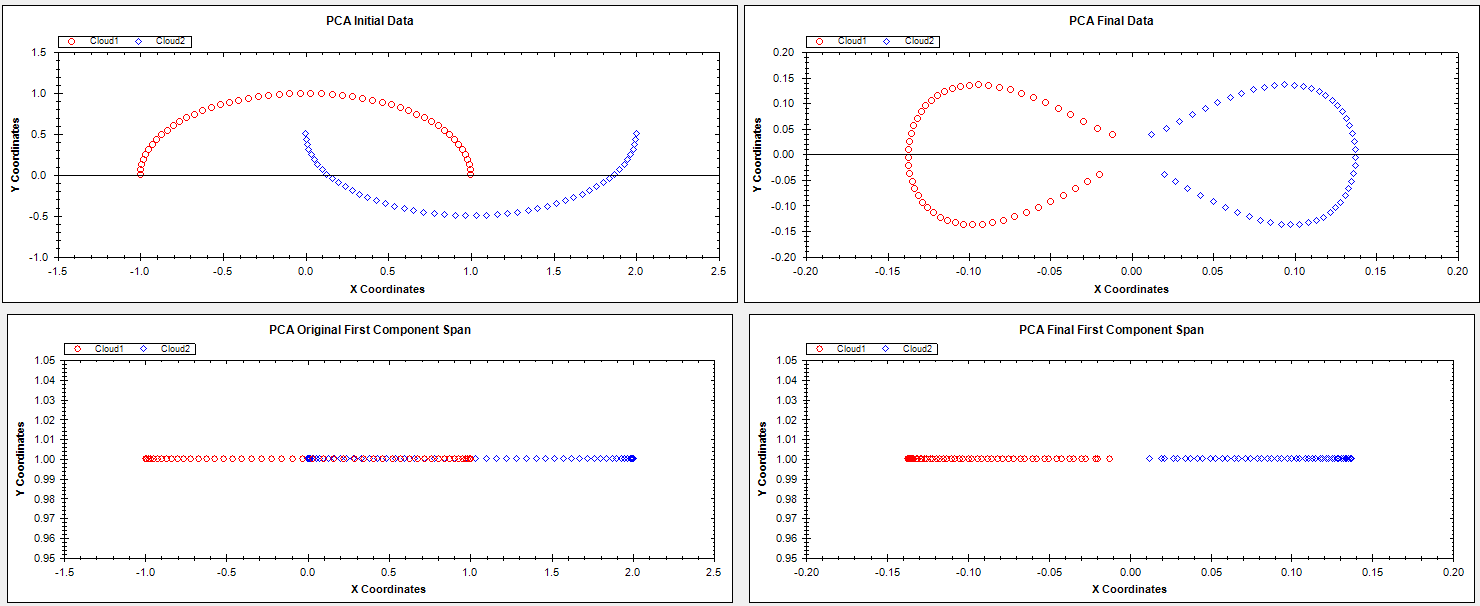
\includegraphics[width=\linewidth]{twomoon1}
\end{figure}

\subsubsection{Cros-validare 10-fold}
Pentru a ne asigura ca algoritmul se comporta corect si in alte situatii, am decis sa facem o cros-validare 10-fold (10-fold crossvalidation). Acest lucru implica urmatoarele: 

-avem 100 de puncte, distribuite in setul de date two-moon

-din acestea, vom alege pe rand, cate 10 puncte, diferite de fiecare data, si vom retine norul din care face parte fiecare

-cu celelalte 90 de puncte vom "antrena" algoritmul pentru a putea proiecta celelalte 10 puncte pe componentele principale respective, in cazul nostru, dorim sa facem proiectarea pe prima componenta principala

-avand cele 90 de puncte proiectate in spatiul nou, putem determina din nou granitele celor 2 nori de puncte, iar mijlocul acestor granite va fi punctul nostru de separare a norilor

-cu punctul de separare gasit, cele 10 puncte proiectate pe prima componenta principala pot fi categorizate: daca se afla in stanga punctului de separare el va fi in norul albastru de puncte, iar daca este la dreapta punctul de separare, va apartine norului rosu

-stiind din ce nori au provenit punctele si in ce nori au fost proiectati, putem verifica eroarea algoritmului pentru cele 10 puncte: $\frac{nr. \text { } puncte \text { } proiectate \text { } gresit}{nr. \text { } puncte \text { } totale}$

-repetam acest proces pana cand toate punctele au fost proiectate, iar eroarea de final este cea cautata

In cazul testelor noastre, eroarea a variat intre 1\% si 4\%, fiind un rezultat foarte bun.

\begin{figure}[H]
\centering
\caption{Exemplu de validare 10-fold}
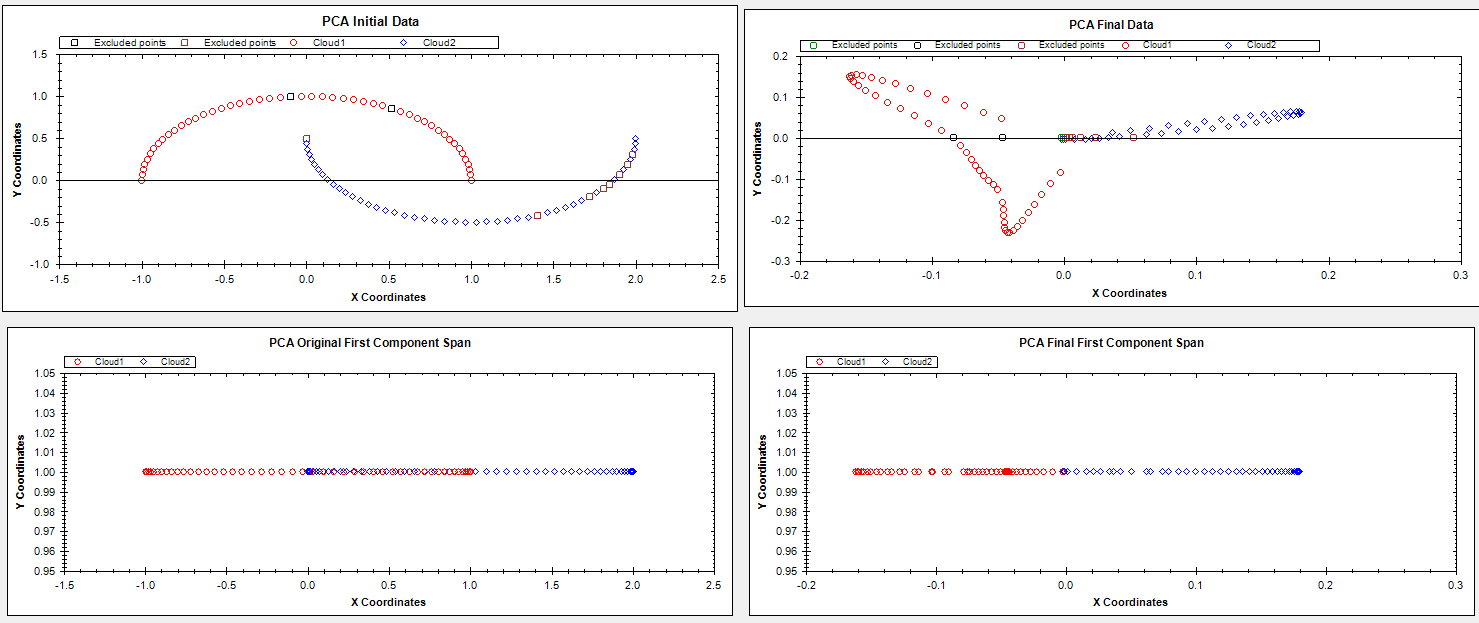
\includegraphics[width=\linewidth]{tenfold1}
\end{figure}

\newpage

\subsection{Aplicatia Eigenfaces}
Dupa ce am realizat testele KPCA, urmatorul pas a fost sa crestem dimensiunile cu care lucram. Mai exact, am inceput sa folosim imagini pentru a vedea cum actioneaza algoritmul PCA pe ele.

Imaginile folosite au fost cele din baza de date Yale, care a fost folosita in multe alte cercetari de genul acesta, continand destui subiecti si destule imagini pentru a putea testa orice algoritm.

Pentru a putea procesa aceste imagini, ele trebuiau sa aiba toate aceeasi dimensiune, in cazul nostru $168 \times 192$, iar fiecare imagine va deveni un rand din matricea care va fi prelucrata de algoritmul PCA.

Fetele rezultate din acest algoritm reprezinta toti vectorii proprii care contribuie la spatiul fetelor intr-un mod semnificativ, si sunt sortati dupa valoarea proprie, si dupa cum se poate observa, aceste imagini devin din ce in ce mai nesemnificative: 

\begin{figure}[H]
\centering
\caption{Primele 10 eigenfaces-uri ale primului subiect}
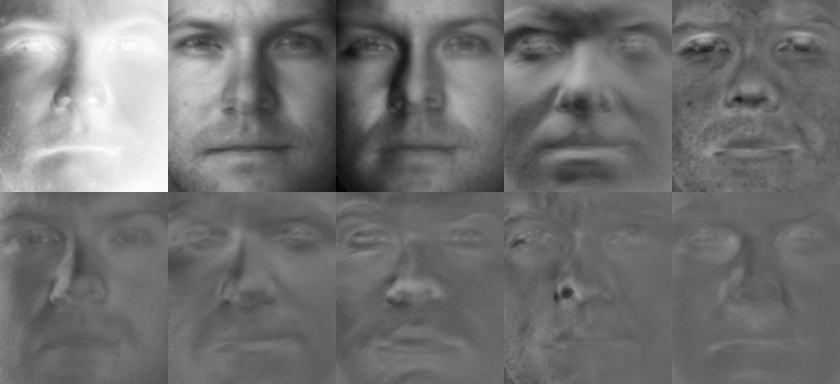
\includegraphics[width=\linewidth]{eigenfaces}
\end{figure}

\subsubsection{Proiectarea unei imagini noi}
Pentru a putea proiecta o imagine noua in spatiul fetelor, tot ce trebuie sa facem este: 

\begin{equation}
X=X-avg(X)
\end{equation}
\begin{equation}
Y=X^T \times E_0
\end{equation}

$X=$ este vectorul imaginii pe care o vom proiecta

$E_0=$ este vectorul propriu asociat valorii proprii maxime

$Y=$ este imaginea proiectata.

\newpage
\subsubsection{Clasificarea unei imagini noi}

Pentru a vedea daca o imagine nou proiectata apartine sau nu setului initial de imagini, avem nevoie mai intai de imaginea proiectata, si de o granita, la fel ca la abordarea KPCA.

Modul prin care vom afla daca o imagine apartine setului este prin calcularea distantei de la aceasta imagine la reprezentarea setului de imagini in spatiul respectiv, iar daca valorea aceasta este mai mica decat granita mentionata mai sus, imaginea va fi clasificata ca va apartine setului initial.

Pentru a afla aceasta distanta, vom efectua urmatoarele operatii:

\begin{equation}
D=W_i-Y
\end{equation}
\begin{equation}
N=\| D_i  \|
\end{equation}
\begin{equation}
v=min(N)
\end{equation}

$W=$ reprezinta fetele setului de date initial proiectate in spatiul fetelor

$D=$ diferenta dintre toate liniile lui $W$ si $Y$ 

$N=$ norma fiecarei linii din $D$

$v=$ este distanta dintre imaginea nou proiectata si spatiul fetelor

Pentru a afla granita care delimiteaza imaginile din spatiul fetelor de celelalte, vom folosi aceleasi operatii ca si mai sus, dar aplicate pe toate imaginile setului initial, si vom cauta $v=avg(N)$, distanta medie dintre toate fetele proiectate si spatiul fetelor. Am ales sa facem acest lucru si sa nu cautam $v=max(N)$ deoarece se poate intampla ca o imagine din setul initial sa aiba distanta fata de spatiul fetelor disproportional mai mare fata de celelalte, si astfel granita de clasificare ar fi prea mare, incluzand orice imagine pe care incercam sa o proiectam.

Acestea fiind zise, am facut urmatorul test: din cele 65 de imagini ale subiectului 1 din baza de date Yale, primele 44 au fost folosite pentru a "antrena" algoritmul, iar ultimele 21 au fost folosite pentru clasificare. Eroarea rezultata a fost de $\sim$ 50\%, imaginile care nu au fost clasificate ca facand parte in set au fost cele in care subiectul are numai jumatate de fata iluminata, numarul acestor imagini fiind $\sim$ 50\% din ele, deci putem trage concluzia ca algoritmul face ceea ce isi propune. 
\end{document}
